%======================================================================
%  Experimental and DFT-Assisted Raman Characterisation of
%  Isolated N-Acetylmuramic Acid
%
%  Sukesh P, Indian Institute of Technology Jodhpur
%
%  Version 2 -- rebuilt on the full archive (227 spectra):
%    - reference spectrum from 22 independent replicate measurements
%    - photostability and laser-damage threshold included
%    - DFT: Gaussian 16, B3LYP-D3BJ/6-311++G(d,p)
%
%  Compile: pdflatex x2.  Items in red need author input before submission.
%======================================================================
\documentclass[preprint,12pt]{elsarticle}

\usepackage{amsmath,amssymb}
\usepackage{graphicx}
\usepackage{booktabs}
\usepackage{xcolor}
\usepackage{lineno}
\usepackage[hidelinks]{hyperref}

\journal{Spectrochimica Acta Part A: Molecular and Biomolecular Spectroscopy}

\newcommand{\wn}{\ensuremath{\mathrm{cm}^{-1}}}
\newcommand{\authorcheck}[1]{\textcolor{red}{[#1]}}

\begin{document}
\begin{frontmatter}

\title{Experimental and DFT-Assisted Raman Characterisation of Isolated
N-Acetylmuramic Acid: Vibrational Assignment, Photostability Limits, and a
Reference Spectrum for Bacterial Cell-Wall Analysis}

\author[iitj]{Sukesh P\corref{cor1}}
\ead{sukeshperiyasamy@gmail.com}
\cortext[cor1]{Corresponding author.}
% \author[iitj]{Supervisor Name}

\affiliation[iitj]{organization={Department of Electrical Engineering,
Indian Institute of Technology Jodhpur},
city={Jodhpur}, postcode={342030}, state={Rajasthan}, country={India}}

\begin{abstract}
N-acetylmuramic acid (MurNAc, NAM) is the defining amino sugar of bacterial
peptidoglycan and underlies many of the vibrational features exploited in
Raman-based microbial identification. Despite this, an experimentally
benchmarked vibrational assignment for the isolated molecule has not been
reported: existing assignments derive either from empirical force-field
treatments of the crystalline monohydrate or from density functional theory
(DFT) calculations validated only indirectly against whole-cell bacterial
spectra. Here we report a reference Raman spectrum of isolated N-acetylmuramic
acid powder, constructed from 22 independent measurements on fresh sample at
785~nm, together with harmonic Raman frequencies computed at the
B3LYP-D3BJ/6-311++G(d,p) level. Forty-one reproducible bands were identified in
the 400--1800~\wn{} fingerprint region, of which thirty were matched to
calculated normal modes with a mean absolute deviation of 9.3~\wn{}, a
root-mean-square deviation of 10.3~\wn{}, and a correlation coefficient of
0.9996. Acquisition conditions were characterised across 227 spectra, yielding a
laser-damage threshold: the sample is spectrally unchanged over ten consecutive
scans at 90\% laser power and 30~s integration, but is destroyed at the same
power with 60~s integration. Normal-mode decomposition resolves two assignments
that could not be reached from the experimental spectrum alone. The intense
872~\wn{} band arises from hydroxymethyl wagging rather than ring breathing, and
the calculated mode falling in the disputed $\sim$730~\wn{} bacterial marker
region originates almost entirely from out-of-plane deformation of the
carboxylic acid hydroxyl group (47.9\% of the mode displacement) with negligible
pyranose ring character (0.5\%). Because this proton is absent in intact
peptidoglycan, where the muramic acid carboxyl is amide-linked to the peptide
stem, the result argues against attributing the bacterial 730~\wn{} band to
muramic acid.
\end{abstract}

\begin{keyword}
Raman spectroscopy \sep density functional theory \sep N-acetylmuramic acid \sep
peptidoglycan \sep vibrational assignment \sep photostability
\end{keyword}

\end{frontmatter}
\linenumbers

%======================================================================
\section{Introduction}
%======================================================================

Raman spectroscopy provides label-free, non-destructive vibrational fingerprints
of biological material with minimal sample preparation, which has made it
attractive for rapid microbial characterisation \cite{wang2022bacteria,
ma2024ecoli}. Bacterial Raman spectra are, however, superpositions of
contributions from proteins, nucleic acids, lipids and the cell wall, so the
interpretation of individual bands depends on the availability of reliable
reference spectra for the constituent molecules.

Among cell-wall components, N-acetylmuramic acid occupies a distinctive
position. Together with N-acetylglucosamine (GlcNAc) it forms the alternating
glycan backbone of peptidoglycan, the polymer that confers mechanical rigidity
on the bacterial cell wall in both Gram-positive and Gram-negative organisms
\cite{vollmer2008}. Unlike GlcNAc, which also occurs widely in eukaryotic
glycans, muramic acid is essentially restricted to bacteria, and its D-lactyl
ether substituent at C-3 is chemically unique to the bacterial cell wall. This
specificity has made it an attractive target for Raman-based and
surface-enhanced Raman (SERS) approaches to bacterial detection.

Raman spectra of structurally related amino sugars have been reported
\cite{she1974raman}, and computational treatments of saccharide Raman spectra
are well established \cite{kaminsky2020saccharides}. Vibrational studies of
muramic acid itself nevertheless remain sparse. Early work combined infrared and
Raman measurements on the crystalline monohydrate with harmonic dynamics based on
empirical force fields \cite{kouach1994}, reaching an average agreement of
approximately 4~\wn{} between observed and calculated frequencies. More
recently, Ma et~al.\ \cite{ma2024ecoli} computed Raman spectra of NAM and GlcNAc
by DFT in order to construct a diagnostic model for \emph{Escherichia coli}. In
that work, however, NAM entered only as an \emph{in silico} spectral component:
the calculated spectrum was compared against whole-cell bacterial measurements,
in which peptidoglycan bands are superimposed on strong protein, lipid and
nucleic acid signals. The NAM assignments were therefore never validated
directly against the isolated molecule.

A further open question concerns the band near 730~\wn{}, among the strongest
and most frequently used features in bacterial SERS spectra. Its origin has been
attributed variously to adenine and related nucleotide degradation products
\cite{premasiri2016origins, kubryk2016origin} and, less frequently, to cell-wall
components. Without a measured spectrum of isolated muramic acid the
peptidoglycan contribution could not be assessed directly.

The present work addresses these gaps. We report a reference Raman spectrum of
isolated N-acetylmuramic acid powder built from independent replicate
measurements, establish the laser conditions under which the material is
spectrally stable, and assign the observed bands using normal-mode decomposition
of a dispersion-corrected DFT calculation.

%======================================================================
\section{Materials and methods}
%======================================================================

\subsection{Materials}

N-acetylmuramic acid (Sigma-Aldrich, product A3007-100MG, lot BCCK5768;
CAS 10597-89-4; synthetic; $\geq$98\% by TLC; white powder; stated residual
methanol $\leq$1~mol/mol) was used as received without further purification or
recrystallisation. The material was supplied in an amber glass bottle and stored
at 2--8~$^{\circ}$C as specified. The molecular weight of 293.27 corresponds to
anhydrous C$_{11}$H$_{19}$NO$_8$, so the material is not a hydrate.

The supplier specification defines five stereocentres but leaves the anomeric
configuration unspecified (SMILES
\texttt{CC(O[C@H]1[C@H](O)[C@@H](CO)OC(O)[C@@H]1NC(C)=O)C(O)=O}; InChI stereo
layer \texttt{/t5-,7+,8-,9-,10-/m1/s1}). The material is therefore an anomeric
mixture rather than a single anomer, as is usual for a reducing sugar. This is
relevant to Section~\ref{sec:unmatched}.

For measurement, a small quantity of powder was deposited directly onto a clean
glass microscope slide. Samples were handled under ambient laboratory conditions
and stored at 2--8~$^\circ$C as supplied.

\subsection{Raman instrumentation}

Spectra were recorded on a B\&W Tek i-Raman Plus system (model BWS465-785H)
coupled to a BAC102-785E Raman microscope, through a 20$\times$ Plan objective.
Excitation was provided by a 785~nm diode laser (Class 3B); the instrument
software reports an emission wavelength of 784.92~nm. Laser power is adjustable
from 0 to 100\% in 1\% increments, and the power settings quoted throughout are
percentages of the instrument maximum.

Three power figures apply to this system and should not be conflated. The laser
safety label states a maximum output of 495~mW, this being the maximum accessible
emission used for hazard classification. The manufacturer specification quotes
455~mW nominal at the laser port and 340~mW nominal exiting the fibre-optic
probe. On the basis of the last of these, the power settings used here correspond
to approximately 17, 136, 238 and 306~mW exiting the probe at 5, 40, 70 and 90\%
respectively.

Power incident on the sample is lower than these figures, because the
measurements reported here were made through a BAC102-785E microscope and a
20$\times$ Plan objective rather than directly from the probe. The transmission
of this optical path was not measured, and the incident power at the sample is
therefore not known in absolute terms. Taking published transmission values for
comparable microscope optics and objectives (approximately 40--65\% in
combination) the power at the sample at the 70\% setting is estimated to lie in
the range 95--155~mW; with a diffraction-limited focus of about 2.4~$\mu$m
diameter for a 20$\times$ objective of numerical aperture 0.40, this corresponds
to an estimated power density of roughly 20--35~mW\,$\mu$m$^{-2}$. These figures
are estimates derived from component specifications and are not measured values.

Power settings are therefore reported throughout as percentages of the instrument
maximum. This is sufficient for reproduction on the same instrument model, and
the nominal figures above allow approximate comparison with other systems, but
absolute power densities should be regarded as indicative only.

Detection used a thermoelectrically cooled high-quantum-efficiency CCD array
(sensor temperature $-2$~$^{\circ}$C) with 2048 pixels. The instrument is
specified for 65--2800~\wn{} at a spectral resolution better than 3.5~\wn{}
(measured at 912~nm using atomic emission lines). Recorded spectra spanned
$-46$ to 2842~\wn{}, of which the 400--1800~\wn{} fingerprint region was
retained for analysis. Spectral sampling varies across the range, from
1.76~\wn{} per pixel at 400~\wn{} to 1.43~\wn{} per pixel at 1800~\wn{}. A dark
spectrum was recorded and subtracted by the instrument software for every
measurement.

\subsection{Measurement design}

A total of 227 spectra were acquired in two sessions and grouped as follows.

\emph{Acquisition-parameter survey} (98 spectra). A full factorial grid of five
integration times (5, 10, 15, 20 and 25~s) and sixteen laser power settings
(5--80\% of nominal output in 5\% steps), two detector readings averaged per
spectrum. Detector saturation did not occur at any condition.

\emph{Replicate sets} (104 spectra). Nine sets, each acquired at a single fixed
condition with the stage moved to fresh powder between every measurement. The
reference spectrum reported here is built from two of these sets, at 70\% and
90\% power, both at 10~s integration with five accumulations, giving 22
independent measurements.

These sets were selected for replicate number and internal consistency rather
than for peak signal-to-noise ratio. Individual sets at longer integration reach
higher SNR --- the 70\%/60~s set attains 789 --- but contain only three spectra
each, and that set also shows the lowest internal agreement of any fresh-spot
set (mean pairwise correlation 0.969). The 10~s sets combine 22 independent
measurements with a mean pairwise correlation of 0.986. For a reference spectrum,
whose purpose is to represent the material reproducibly rather than to maximise
signal in any single measurement, replication and agreement were judged the more
important criteria. The three longer-integration sets (30 and 60~s, 11 spectra,
SNR up to 789) were instead used where high SNR is decisive, namely in verifying
weak bands (Section~2.6).

\emph{Photostability series} (10 spectra). Ten consecutive scans at 90\% power
and 30~s integration acquired without moving the stage.

\emph{Laser-damage series} (10 spectra). Two sets at 90\% power and 60~s
integration, one on a single spot and one on fresh spots. These spectra are
reported in Section~\ref{sec:photostab} and excluded from all vibrational
analysis.

\emph{Substrate blanks} (5 spectra). Empty glass slide.
\authorcheck{These blanks were recorded at 5\% power and 5~s only, which does
not match the sample conditions. Three blanks at the reference condition should
be added before submission.}

\subsection{Spectral processing}

All spectra were processed through an identical pipeline. Dark-subtracted
intensities were interpolated onto a uniform 1~\wn{} grid spanning
400--1800~\wn{}. Baseline contributions from the substrate and residual
fluorescence were removed by asymmetric least-squares fitting \cite{eilers2005}
with smoothing parameter $\lambda = 10^{5}$, asymmetry $p = 0.001$ and ten
iterations. Baseline-corrected spectra were smoothed with a Savitzky--Golay
filter \cite{savitzky1964} (window 11 points, third-order polynomial), chosen to
suppress detector noise without measurable distortion of band positions or
widths, and min--max normalised. Signal-to-noise ratio was estimated as the
ratio of maximum band intensity above the median to the noise standard deviation
determined from successive differences above 1750~\wn{}. Processing used Python
with NumPy, SciPy and pandas.

\subsection{Band identification}

Band positions were located by prominence-based peak detection on the averaged
reference spectrum. Distinguishing genuine weak bands from correlated processing
artefacts requires care: baseline correction and smoothing generate reproducible
residual structure, so a feature appearing consistently across spectra is not by
itself evidence that it is real. Each candidate was therefore evaluated against
the local noise level, estimated from successive differences within a
$\pm$50~\wn{} window, using two independent criteria --- peak prominence and
peak height above the local median --- each required to exceed three times the
local noise.

Bands satisfying both criteria are reported as high confidence. Bands satisfying
only one were additionally tested against the independent long-integration
dataset (30 and 60~s, signal-to-noise ratio up to 796) and promoted to high
confidence where they were confirmed there; otherwise they are reported as
tentative. Five candidate features, at 424, 558, 800, 901 and 1629~\wn{}, failed
both criteria and are not reported. A reproducibility value is quoted for each
band, defined as the fraction of the 22 individual spectra in which a peak was
independently detected within $\pm$4~\wn{} of the mean position.

\subsection{DFT calculations}

Geometry optimisation and harmonic vibrational frequency calculations were
performed with Gaussian~16, Revision C.01 \cite{gaussian16} at the B3LYP level
\cite{becke1993,lee1988} using the 6-311++G(d,p) basis set, with Grimme's D3
dispersion correction and Becke--Johnson damping \cite{grimme2011} and Raman
activities requested. Optimisation used tight convergence criteria with
analytically computed initial force constants, an ultrafine integration grid,
and tight SCF convergence with quadratic convergence enabled
(\texttt{opt=(calcfc,tight) freq=raman int=ultrafine scf=(tight,xqc)}).
Calculations treated the isolated molecule in the gas phase; no implicit
solvation model was applied.

The starting geometry was the $\beta$ anomer of N-acetylmuramic acid taken from
the PubChem 3D conformer record (CID~5462244). The optimisation converged to a
stationary point and the job reached normal termination. The optimised structure
comprises 39 atoms (C$_{11}$H$_{19}$NO$_8$) and yielded 111 normal modes, none
imaginary, confirming a true minimum on the potential energy surface. Harmonic
wavenumbers were scaled by 0.980 below 1800~\wn{} and 0.967 above, following the
scheme applied by Ma et~al.\ \cite{ma2024ecoli}, permitting direct comparison
with the only other modern DFT treatment of this molecule.

Simulated Raman intensities were obtained from the computed Raman activities
$S_i$ using the standard Placzek expression,
\begin{equation}
I_i \;\propto\; \frac{(\nu_0-\nu_i)^4\,S_i}
{\nu_i\left[1-\exp\!\left(-hc\nu_i/k_BT\right)\right]},
\end{equation}
with $\nu_0$ the excitation wavenumber and $T = 298.15$~K, then convolved with
Lorentzian line shapes of 10~\wn{} full width at half maximum.

Mode characters were determined from the calculated Cartesian displacement
vectors. Bond connectivity was established from interatomic distances using
covalent radii, and for each normal mode the fractional contribution of every
atom, of the pyranose ring, and of individual bond-stretching coordinates was
evaluated from mass-weighted displacements. This provides a quantitative and
reproducible basis for the assignments in Table~\ref{tab:comparison}. It is not
equivalent to a full potential energy distribution analysis, and principal
assignments should be confirmed by inspection of the normal-mode animations.

%======================================================================
\section{Results and discussion}
%======================================================================

\subsection{Optimised molecular geometry}

The DFT-optimised structure is shown in Figure~\ref{fig:structure}. The pyranose
ring adopts the expected $^4C_1$ chair conformation, with the acetamido group at
C-2, the D-lactyl ether at C-3 and the hydroxymethyl group at C-5. Optimised
Cartesian coordinates are given in the Supplementary Material.

\begin{figure}[htbp]
\centering
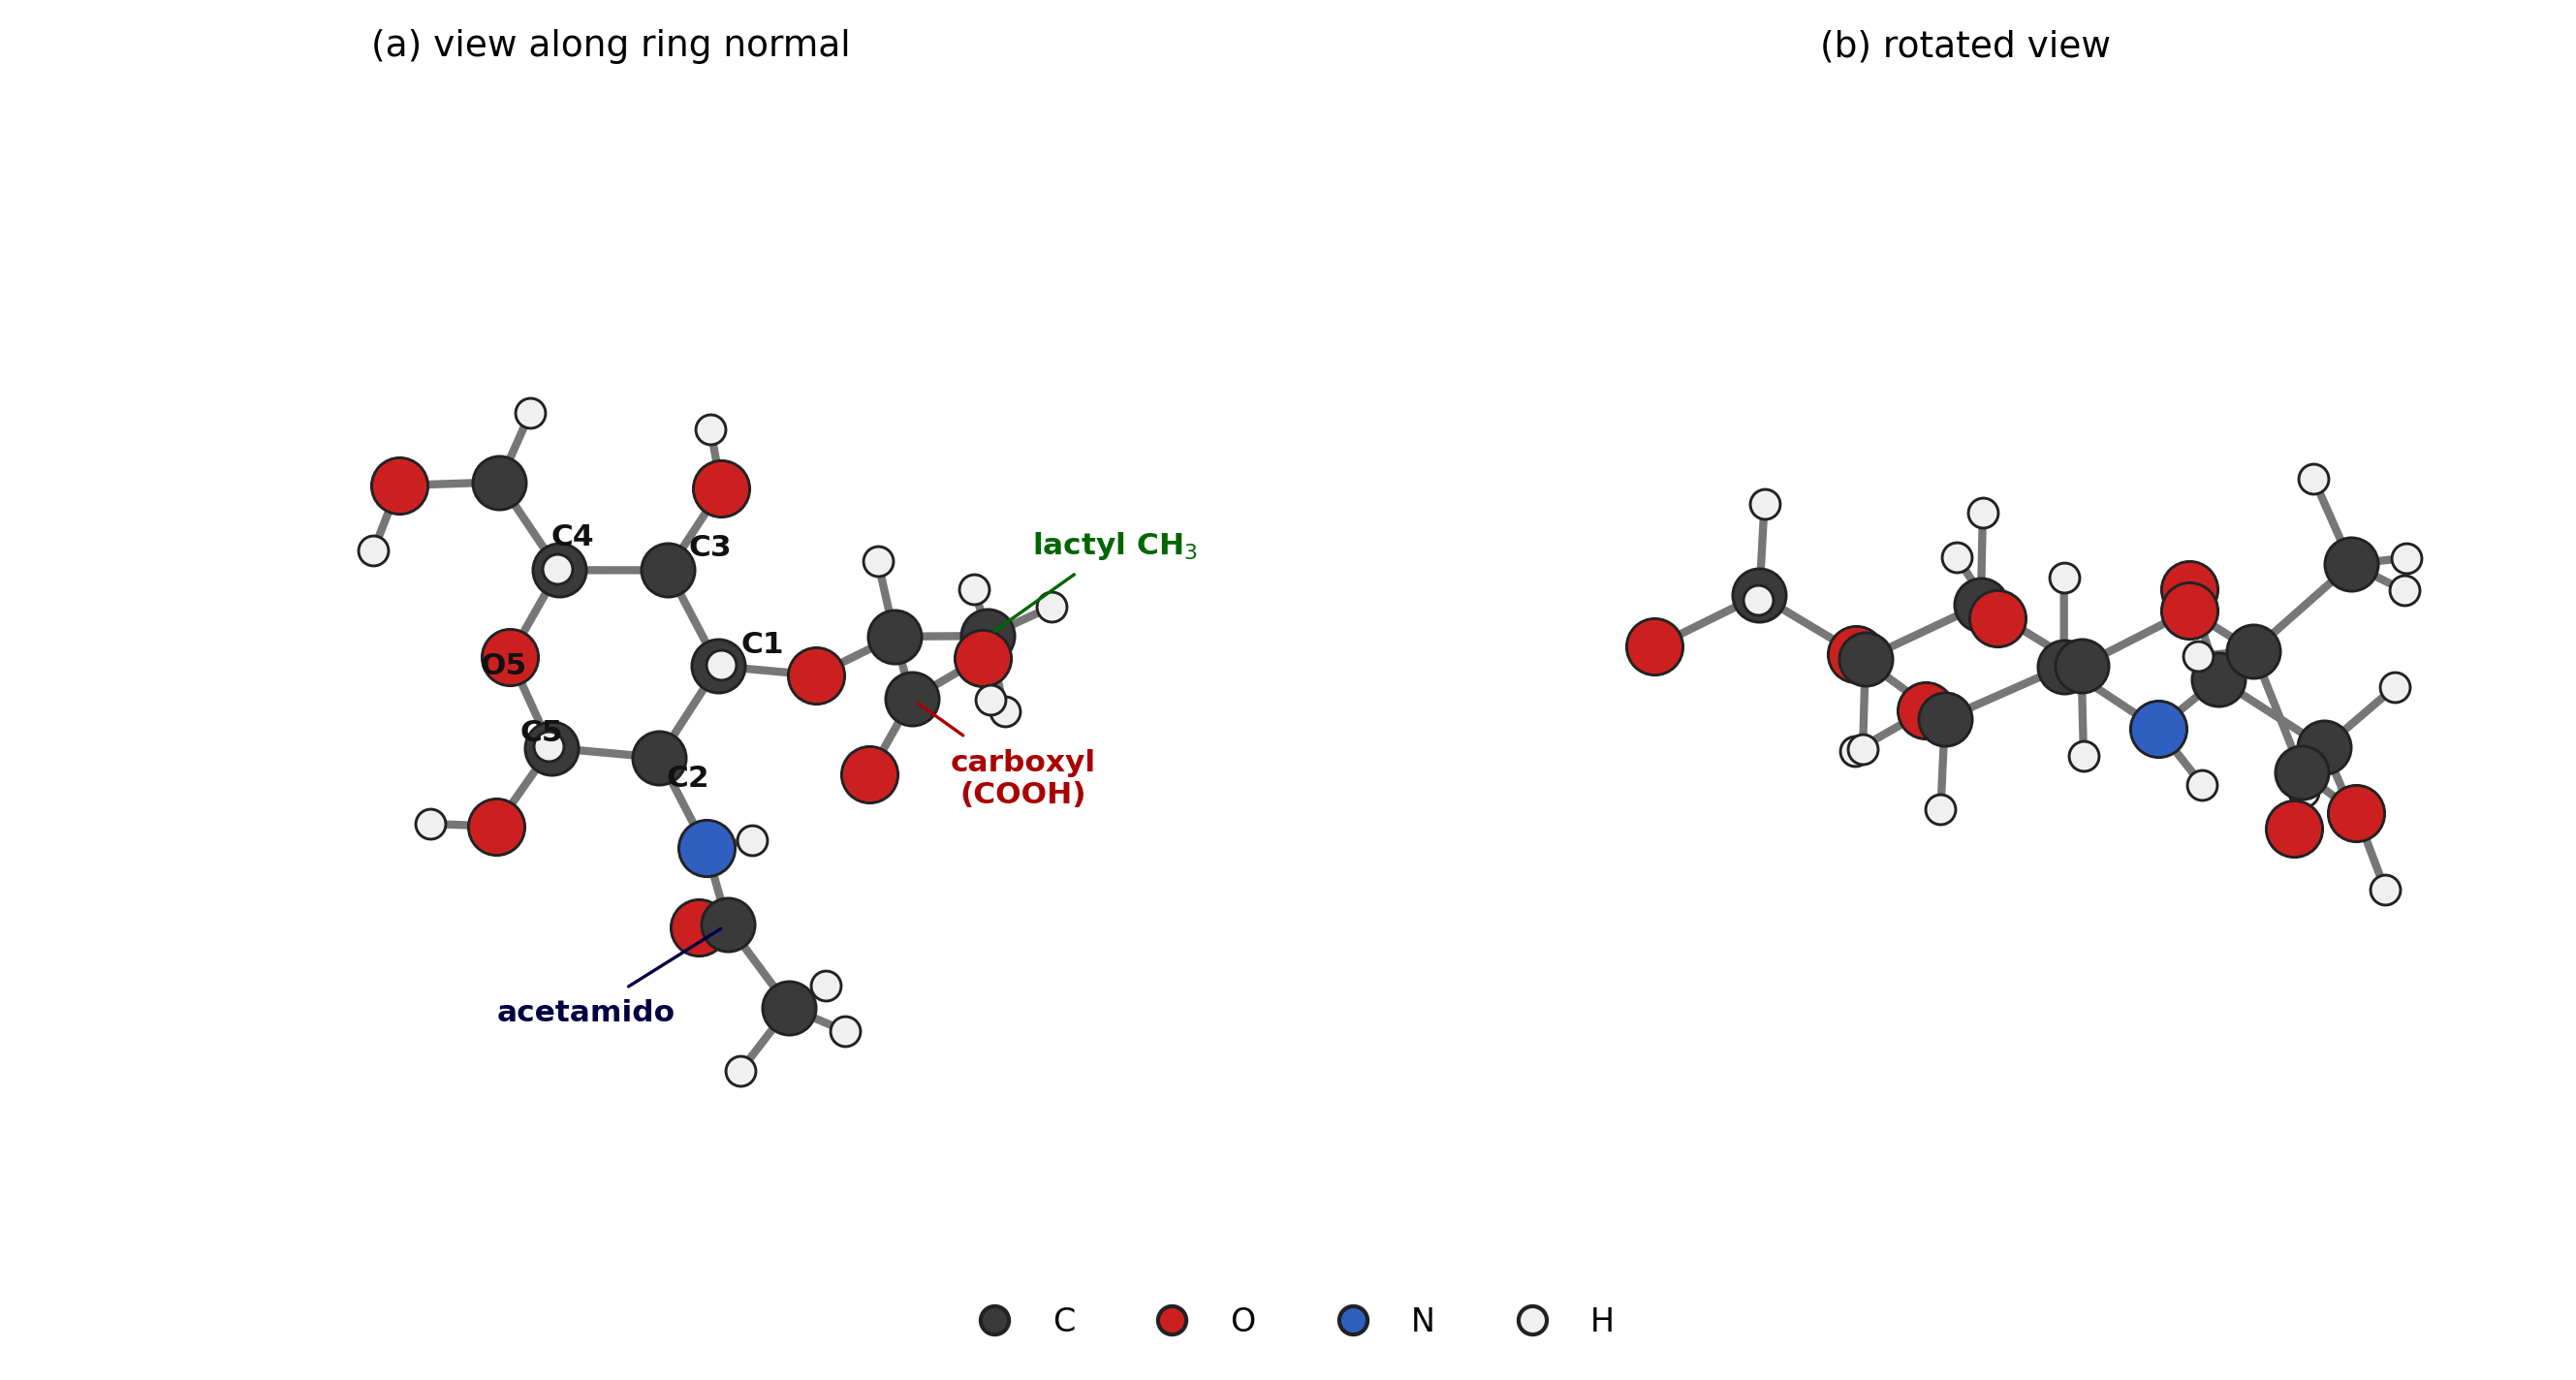
\includegraphics[width=0.92\linewidth]{figures/fig1_structure.png}
\caption{DFT-optimised geometry of $\beta$-N-acetylmuramic acid at the
B3LYP-D3BJ/6-311++G(d,p) level. (a) View along the pyranose ring normal, with
ring carbons and the three substituent groups labelled. (b) Rotated view showing
the $^4C_1$ chair conformation. The D-lactyl ether at C-3 and its terminal
carboxyl group distinguish muramic acid from N-acetylglucosamine.}
\label{fig:structure}
\end{figure}

\subsection{Acquisition conditions}

Figure~\ref{fig:optim} summarises the signal-to-noise ratio across the
acquisition grid. SNR increases monotonically with both integration time and
laser power over the ranges examined, reaching approximately 287 at 25~s and
75\% power. Band positions are unchanged across the entire grid: the 930 and
1451~\wn{} bands remain within $\pm$1~\wn{} of their mean positions from 5\% to
80\% power, and the full width at half maximum of the 930~\wn{} band stays
between 9 and 11~\wn{}. No broad carbonaceous background develops and no band
structure is lost.

\begin{figure}[htbp]
\centering

\includegraphics[width=\linewidth]{figures/fig3_optimisation.png}
\caption{Acquisition-parameter survey for N-acetylmuramic acid powder across 98
spectra. (a) Signal-to-noise ratio across five integration times and sixteen
laser power settings. (b) Signal-to-noise ratio as a function of laser power at
each integration time.}
\label{fig:optim}
\end{figure}

We note that in this survey the power was stepped in ascending order within each
series, so laser power and cumulative exposure are not statistically separable.
The photostability measurements described next were designed to address this
directly.

\subsection{Photostability and the laser-damage threshold}
\label{sec:photostab}

Figure~\ref{fig:photostab} shows two contrasting series acquired without moving
the stage.

At 90\% power and 30~s integration the spectrum is unchanged over ten
consecutive scans. The normalised intensity of the strongest band, at
930~\wn{}, varies by less than 2\% across the series, and the spectra overlay
almost exactly.

At the same power with 60~s integration the material is destroyed. The
intensity of the 930~\wn{} band falls monotonically from 0.44 to 0.23 over five
consecutive scans, the characteristic sharp features at 872, 930 and 956~\wn{}
collapse, and the spectrum degrades towards a broad, poorly structured profile.
Correlation with the reference spectrum falls to $r = 0.06$--$0.31$. The same
behaviour is seen when fresh spots are used at this condition.

\begin{figure}[htbp]
\centering
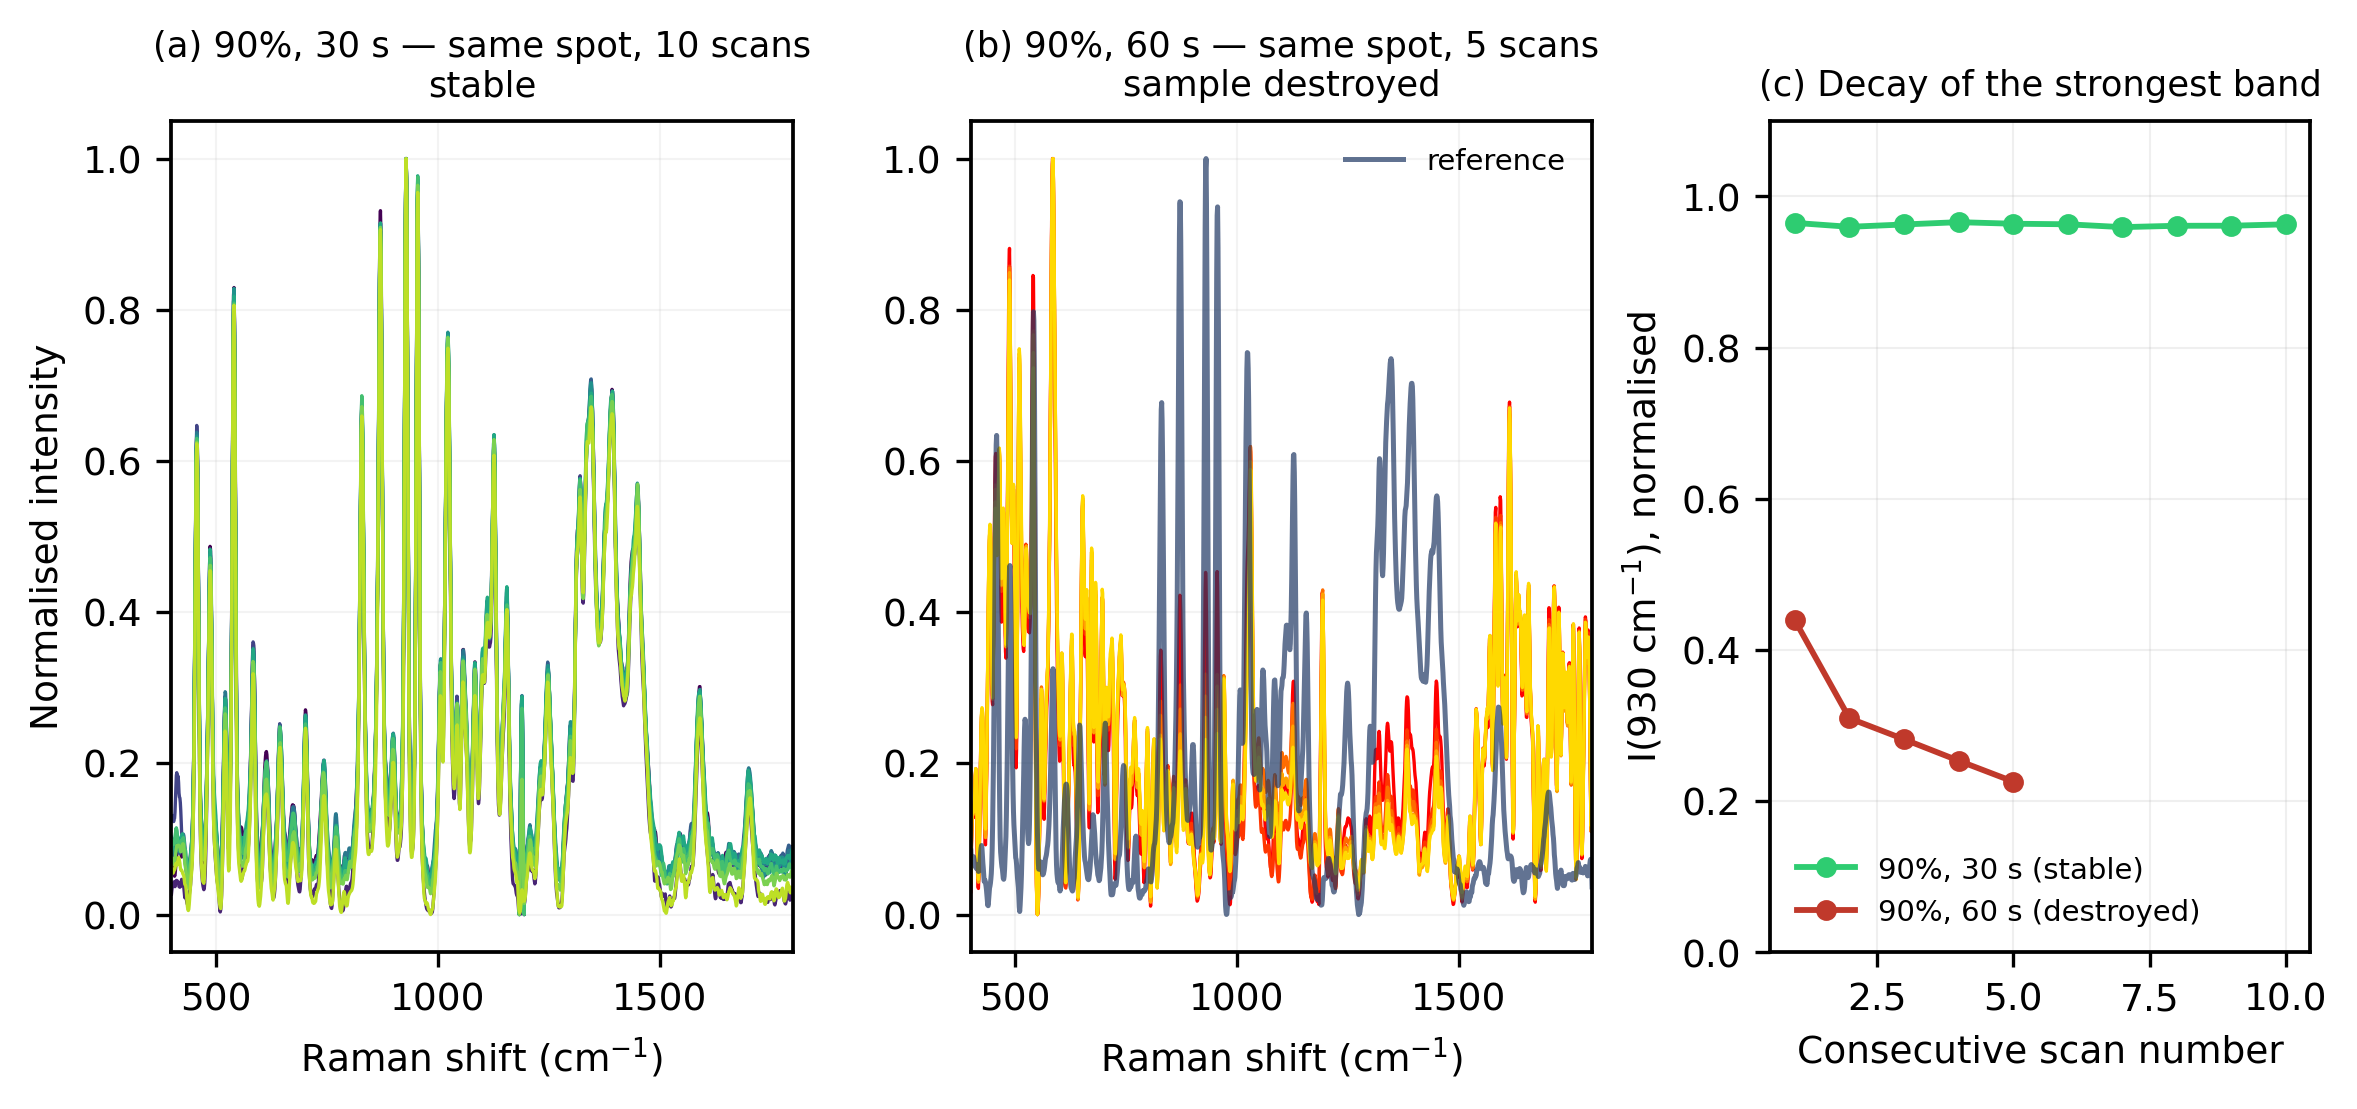
\includegraphics[width=\linewidth]{figures/fig4_photostability.png}
\caption{Photostability of N-acetylmuramic acid powder under 785~nm excitation.
(a) Ten consecutive scans at 90\% laser power and 30~s integration, same spot:
the spectra are indistinguishable. (b) Five consecutive scans at 90\% power and
60~s integration, same spot, with the reference spectrum shown for comparison:
the sample is destroyed. (c) Normalised intensity of the 930~\wn{} band across
consecutive scans for both conditions.}
\label{fig:photostab}
\end{figure}

Taken with the acquisition survey, these measurements define a working envelope
for this material at 785~nm through a 20$\times$ objective:

\begin{center}
\begin{tabular}{lc}
\toprule
Condition & Outcome \\
\midrule
$\leq$80\% power, $\leq$25~s & stable \\
70\% power, 30~s & stable ($r = 0.977$) \\
70\% power, 60~s & stable ($r = 0.970$) \\
90\% power, 30~s & stable over 10 consecutive scans \\
\textbf{90\% power, 60~s} & \textbf{sample destroyed} \\
\bottomrule
\end{tabular}
\end{center}

Reporting this limit explicitly seems worthwhile: carbohydrate powders are often
assumed to tolerate near-infrared excitation indefinitely, and the transition
here is abrupt rather than gradual.

The threshold is expressed here in terms of instrument settings, which permits
exact reproduction on the same instrument. In absolute terms, and using the
estimates given in Section~2.2, the damaging condition corresponds to a power
density of order 25--45~mW\,$\mu$m$^{-2}$ sustained for 60~s, while the same
power density for 30~s produced no detectable change. We emphasise that these
absolute values are estimated from component specifications rather than measured,
and that the exposure duration is as important as the power: the sample tolerated
ten consecutive 30~s exposures at the same power that destroyed it in a single
60~s exposure.

\subsection{Reference Raman spectrum}

The reference spectrum, constructed as the mean of 22 independent measurements
on fresh sample, is shown in Figure~\ref{fig:ref}. The mean pairwise correlation
coefficient among the contributing spectra is 0.986, and the two contributing
sets --- acquired at 70\% and 90\% power --- agree with one another at
$r = 0.992$, confirming that band positions and relative intensities are
independent of laser power within the stable regime.

Forty-one bands satisfy the confidence criteria in the 400--1800~\wn{} region:
32 high confidence and 9 tentative. Two further bands, at 1007 and 1112~\wn{},
were promoted from tentative to high confidence by independent confirmation in
the long-integration dataset. The most intense features occur at 930, 956, 872,
831, 1024 and 542~\wn{}.

\begin{figure}[htbp]
\centering
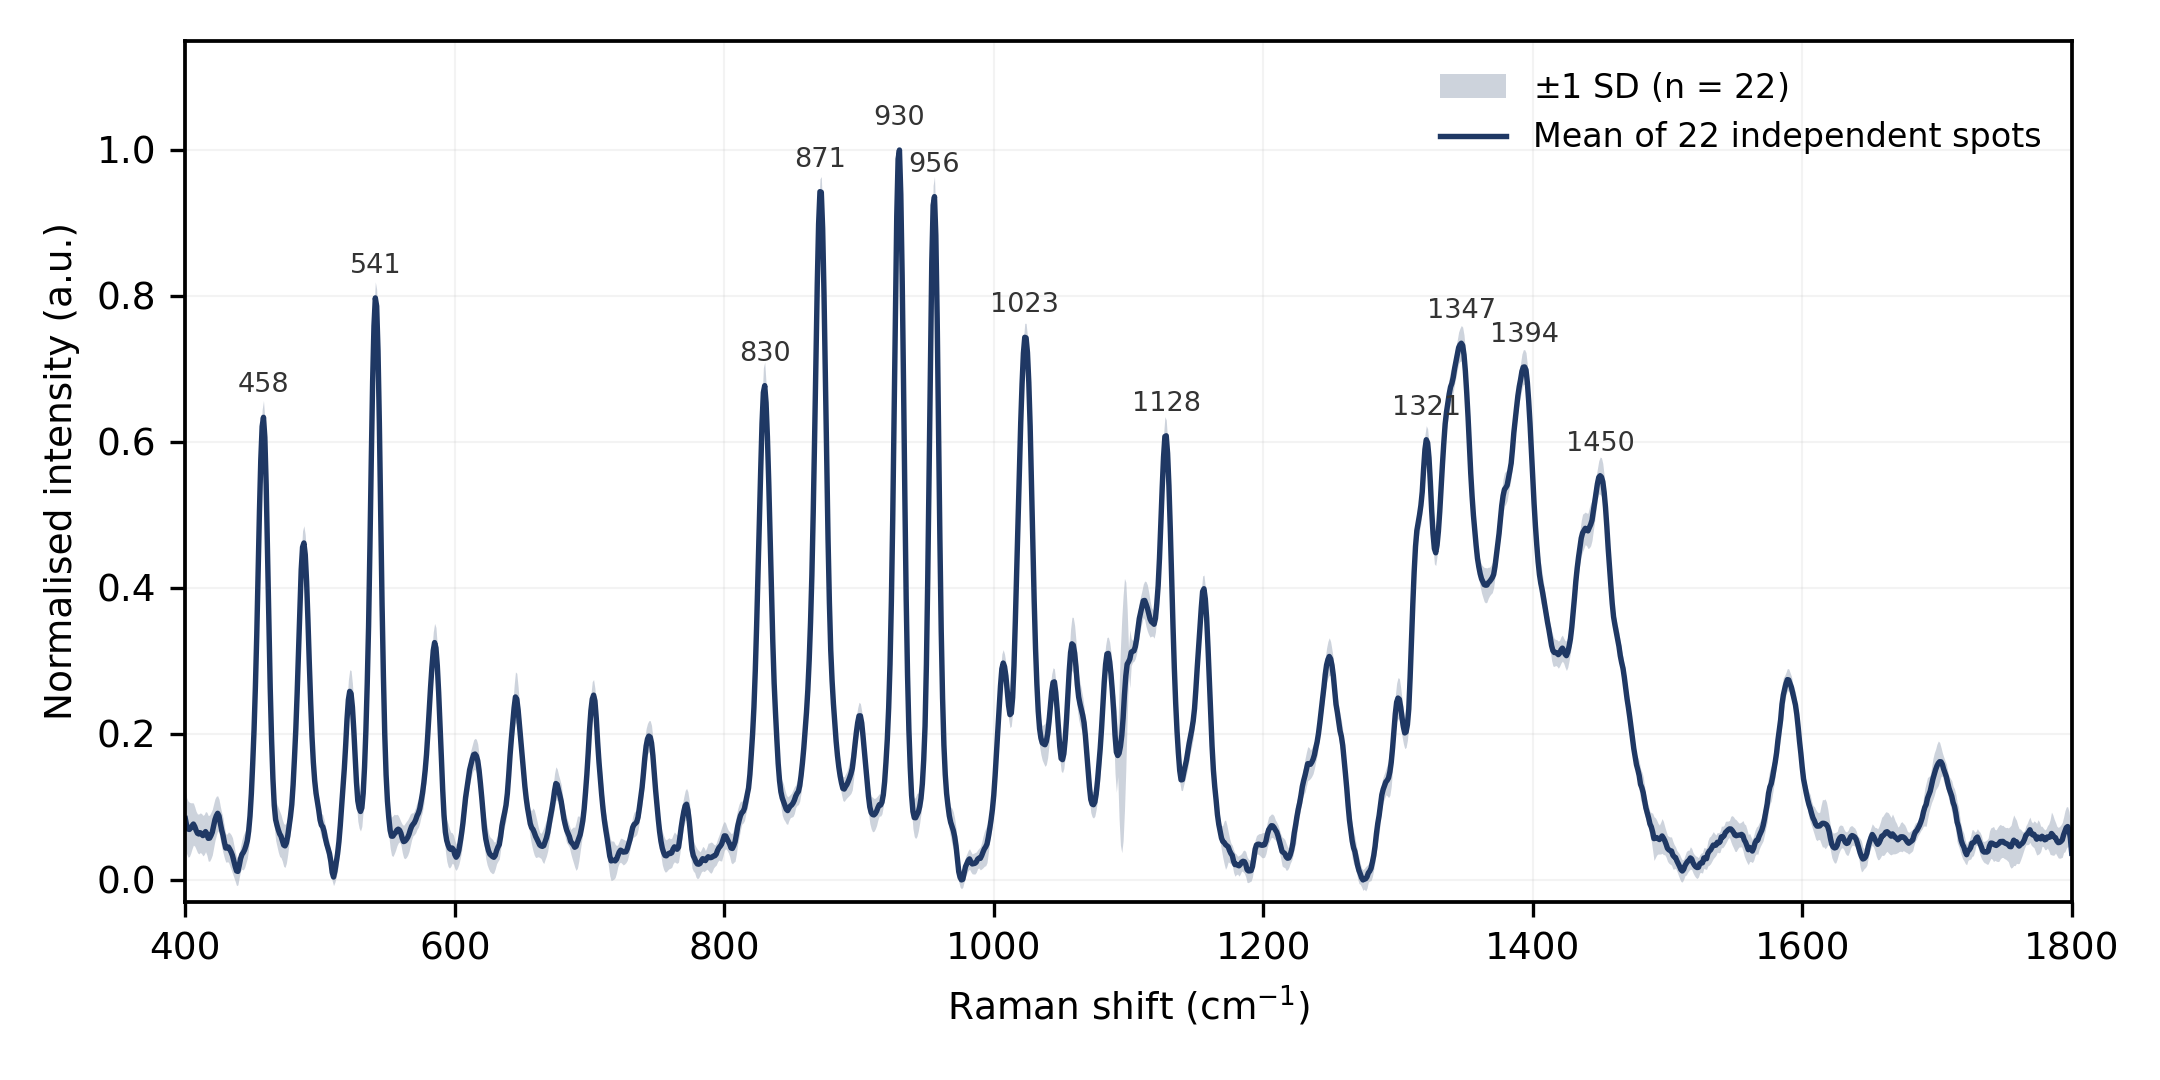
\includegraphics[width=\linewidth]{figures/fig2_reference.png}
\caption{Reference Raman spectrum of isolated N-acetylmuramic acid powder.
Solid line: mean of 22 independent measurements on fresh sample at 785~nm.
Shaded band: $\pm$1 standard deviation. Principal band positions are labelled in
\wn{}.}
\label{fig:ref}
\end{figure}

The spectrum divides into four regions. Below 700~\wn{} the bands at 458, 488,
523, 542, 585 and 646~\wn{} arise from skeletal bending and ring torsional
motions of the pyranose framework. Between 700 and 1000~\wn{} the strong
features at 831, 872, 930 and 956~\wn{} correspond to ring deformation,
hydroxymethyl motion and ring breathing with coupled C--C--O stretching; the
prominence of this region is characteristic of pyranose sugars. The
1000--1200~\wn{} region, containing bands at 1024, 1059, 1085, 1128 and
1157~\wn{}, is dominated by C--O and C--C stretching of the ring together with
C--O--H bending. Above 1200~\wn{} the bands at 1321, 1346, 1395 and 1451~\wn{}
reflect C--H bending, methyl umbrella and methylene scissoring deformations, the
last carrying substantial contribution from the lactyl methyl group.

\subsection{Simulated spectrum}

The simulated Raman spectrum obtained after scaling, intensity conversion and
Lorentzian broadening is shown in Figure~\ref{fig:sim}. Sixty-seven of the 111
computed modes fall within the 400--1800~\wn{} window examined experimentally.

\begin{figure}[htbp]
\centering
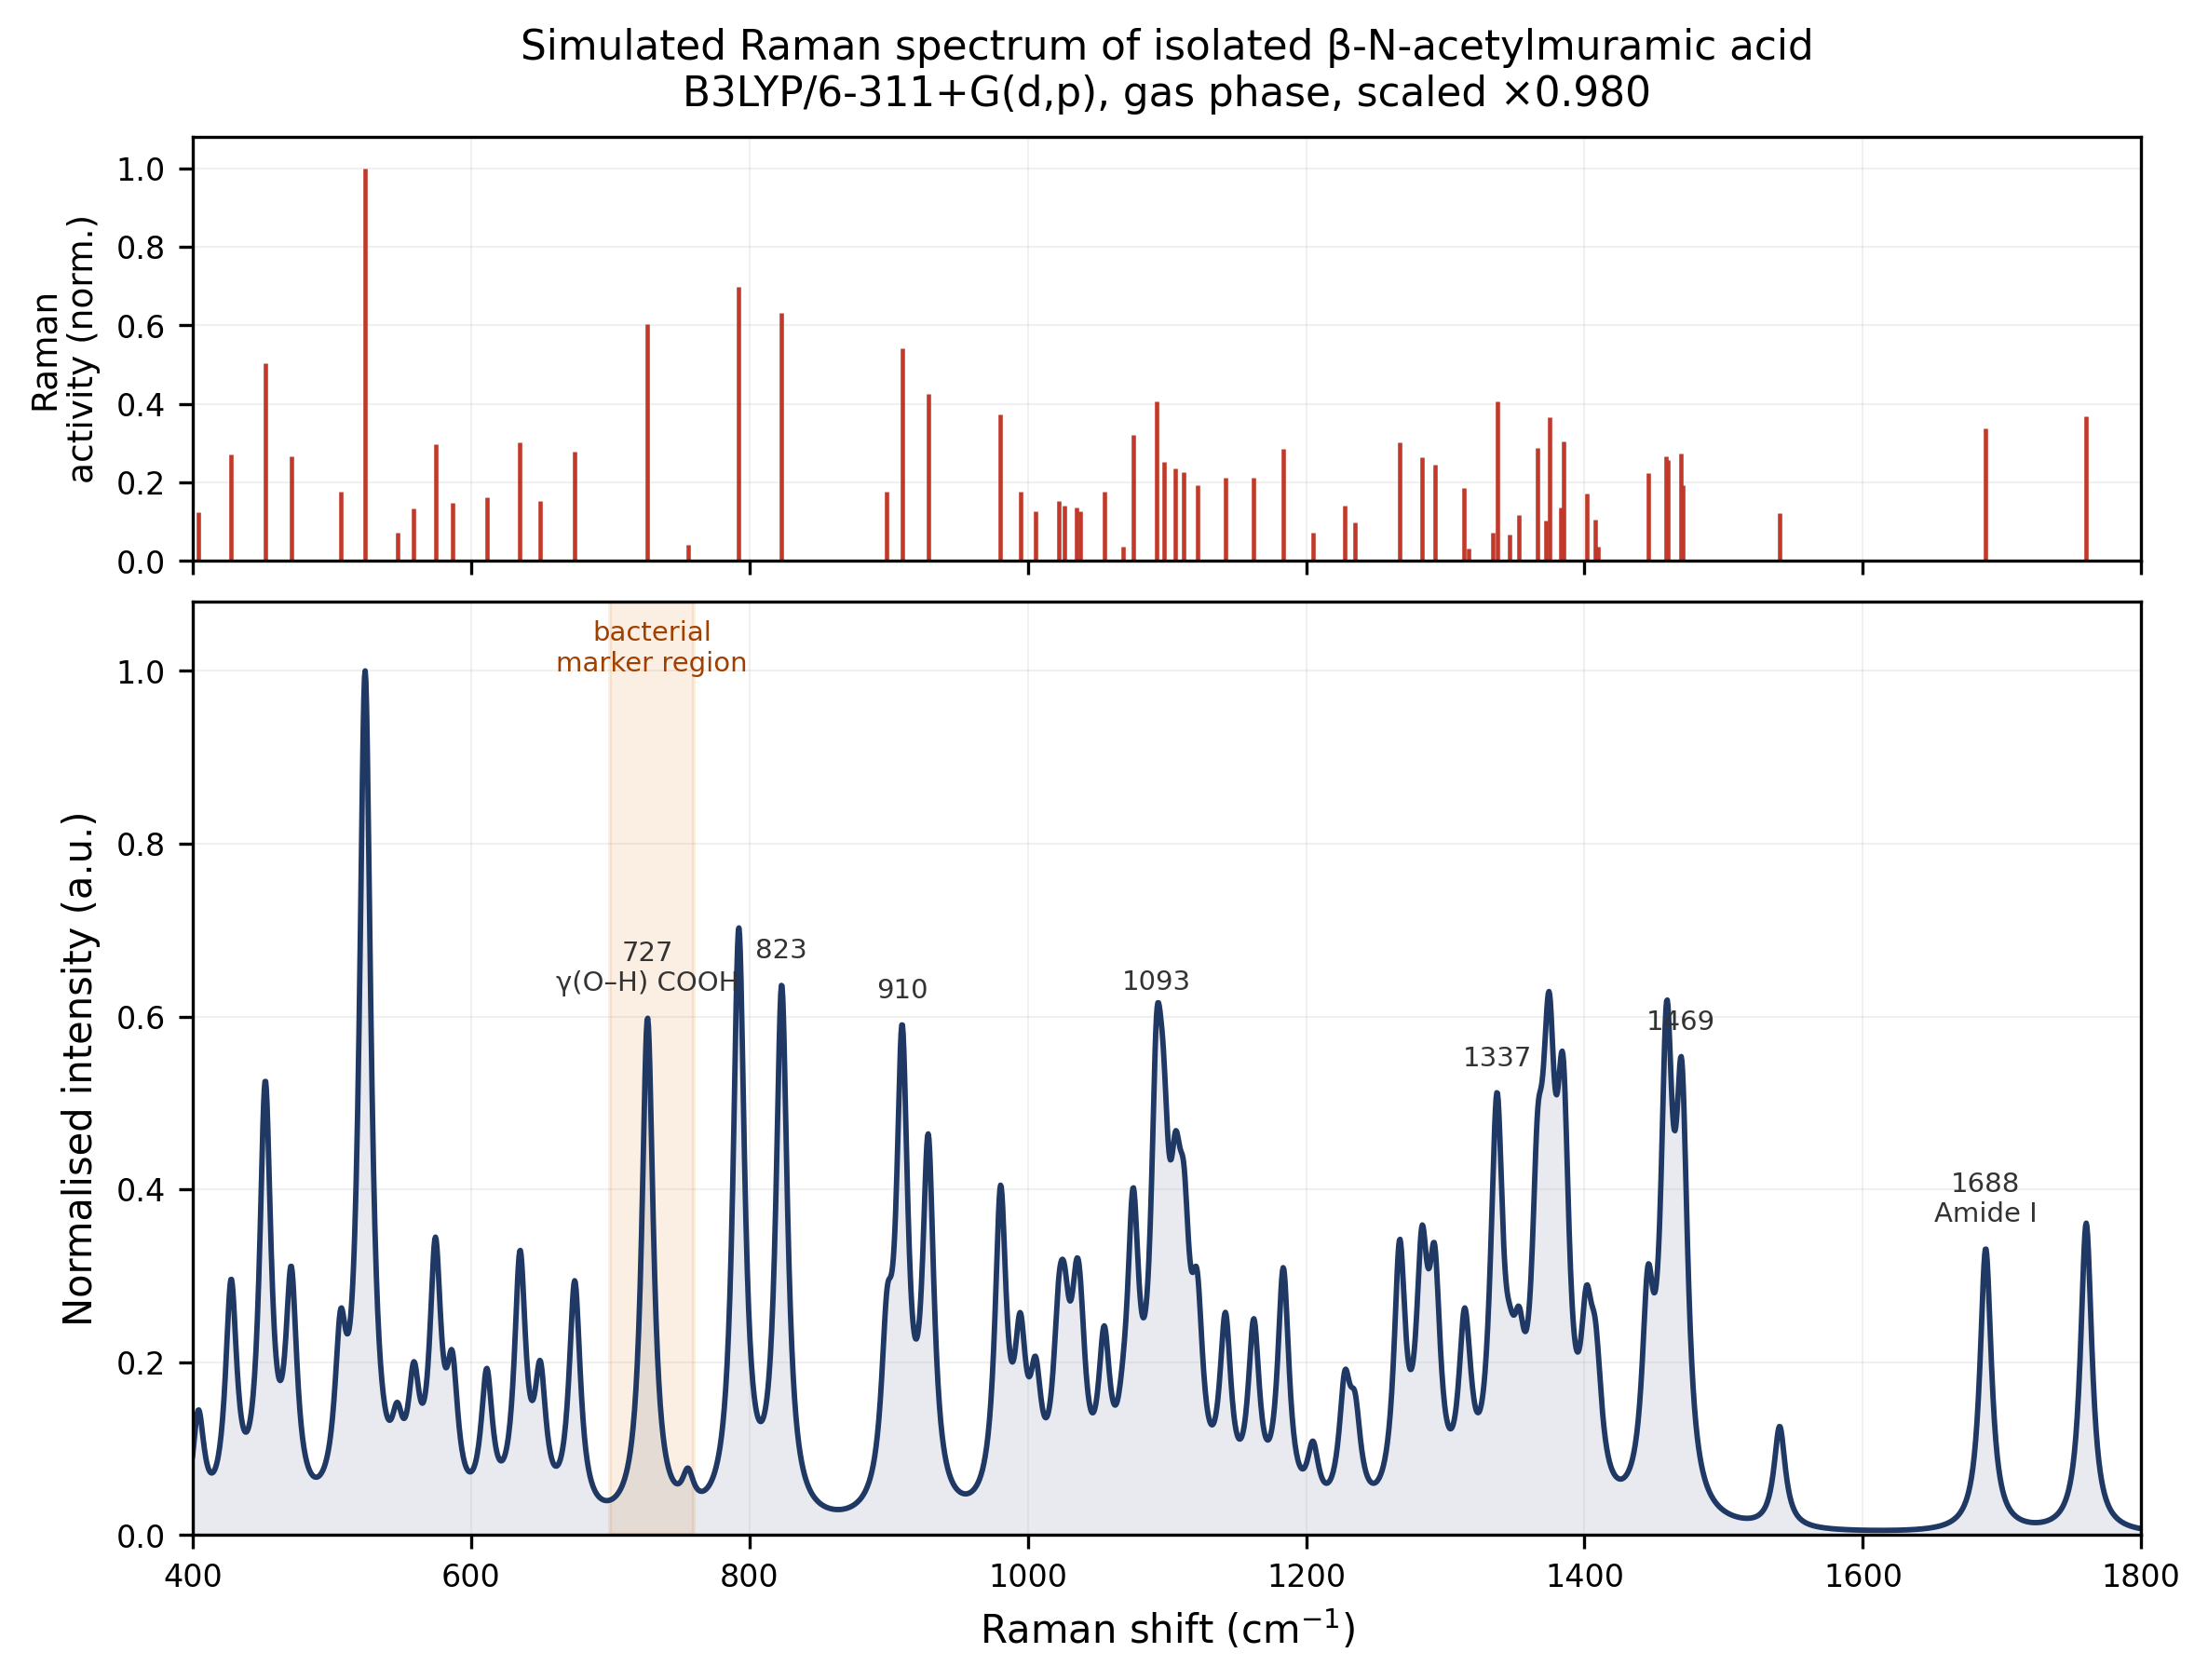
\includegraphics[width=\linewidth]{figures/fig5_simulated.png}
\caption{Simulated Raman spectrum of isolated $\beta$-N-acetylmuramic acid
computed at the B3LYP-D3BJ/6-311++G(d,p) level. Upper panel: scaled harmonic
frequencies with normalised Raman activities. Lower panel: Lorentzian-broadened
spectrum (FWHM 10~\wn{}).}
\label{fig:sim}
\end{figure}

\subsection{Comparison of experimental and calculated frequencies}

Thirty of the forty-one observed bands were matched to calculated normal modes
within a tolerance of $\pm$18~\wn{}, selecting in each case the candidate of
highest Raman activity. The comparison appears in Table~\ref{tab:comparison} and
is displayed in Figure~\ref{fig:overlay}.

Agreement is good. The mean absolute deviation is 9.3~\wn{}, the root-mean-square
deviation 10.3~\wn{}, and the largest individual deviation 17.2~\wn{}. The
correlation between observed and calculated wavenumbers is 0.9996. The mean
signed deviation is $+1.6$~\wn{}, indicating no strong systematic bias after
scaling. Restricting the comparison to high-confidence bands alone gives
essentially the same result (MAE 9.2~\wn{}, RMSE 10.2~\wn{}).

\begin{figure}[htbp]
\centering
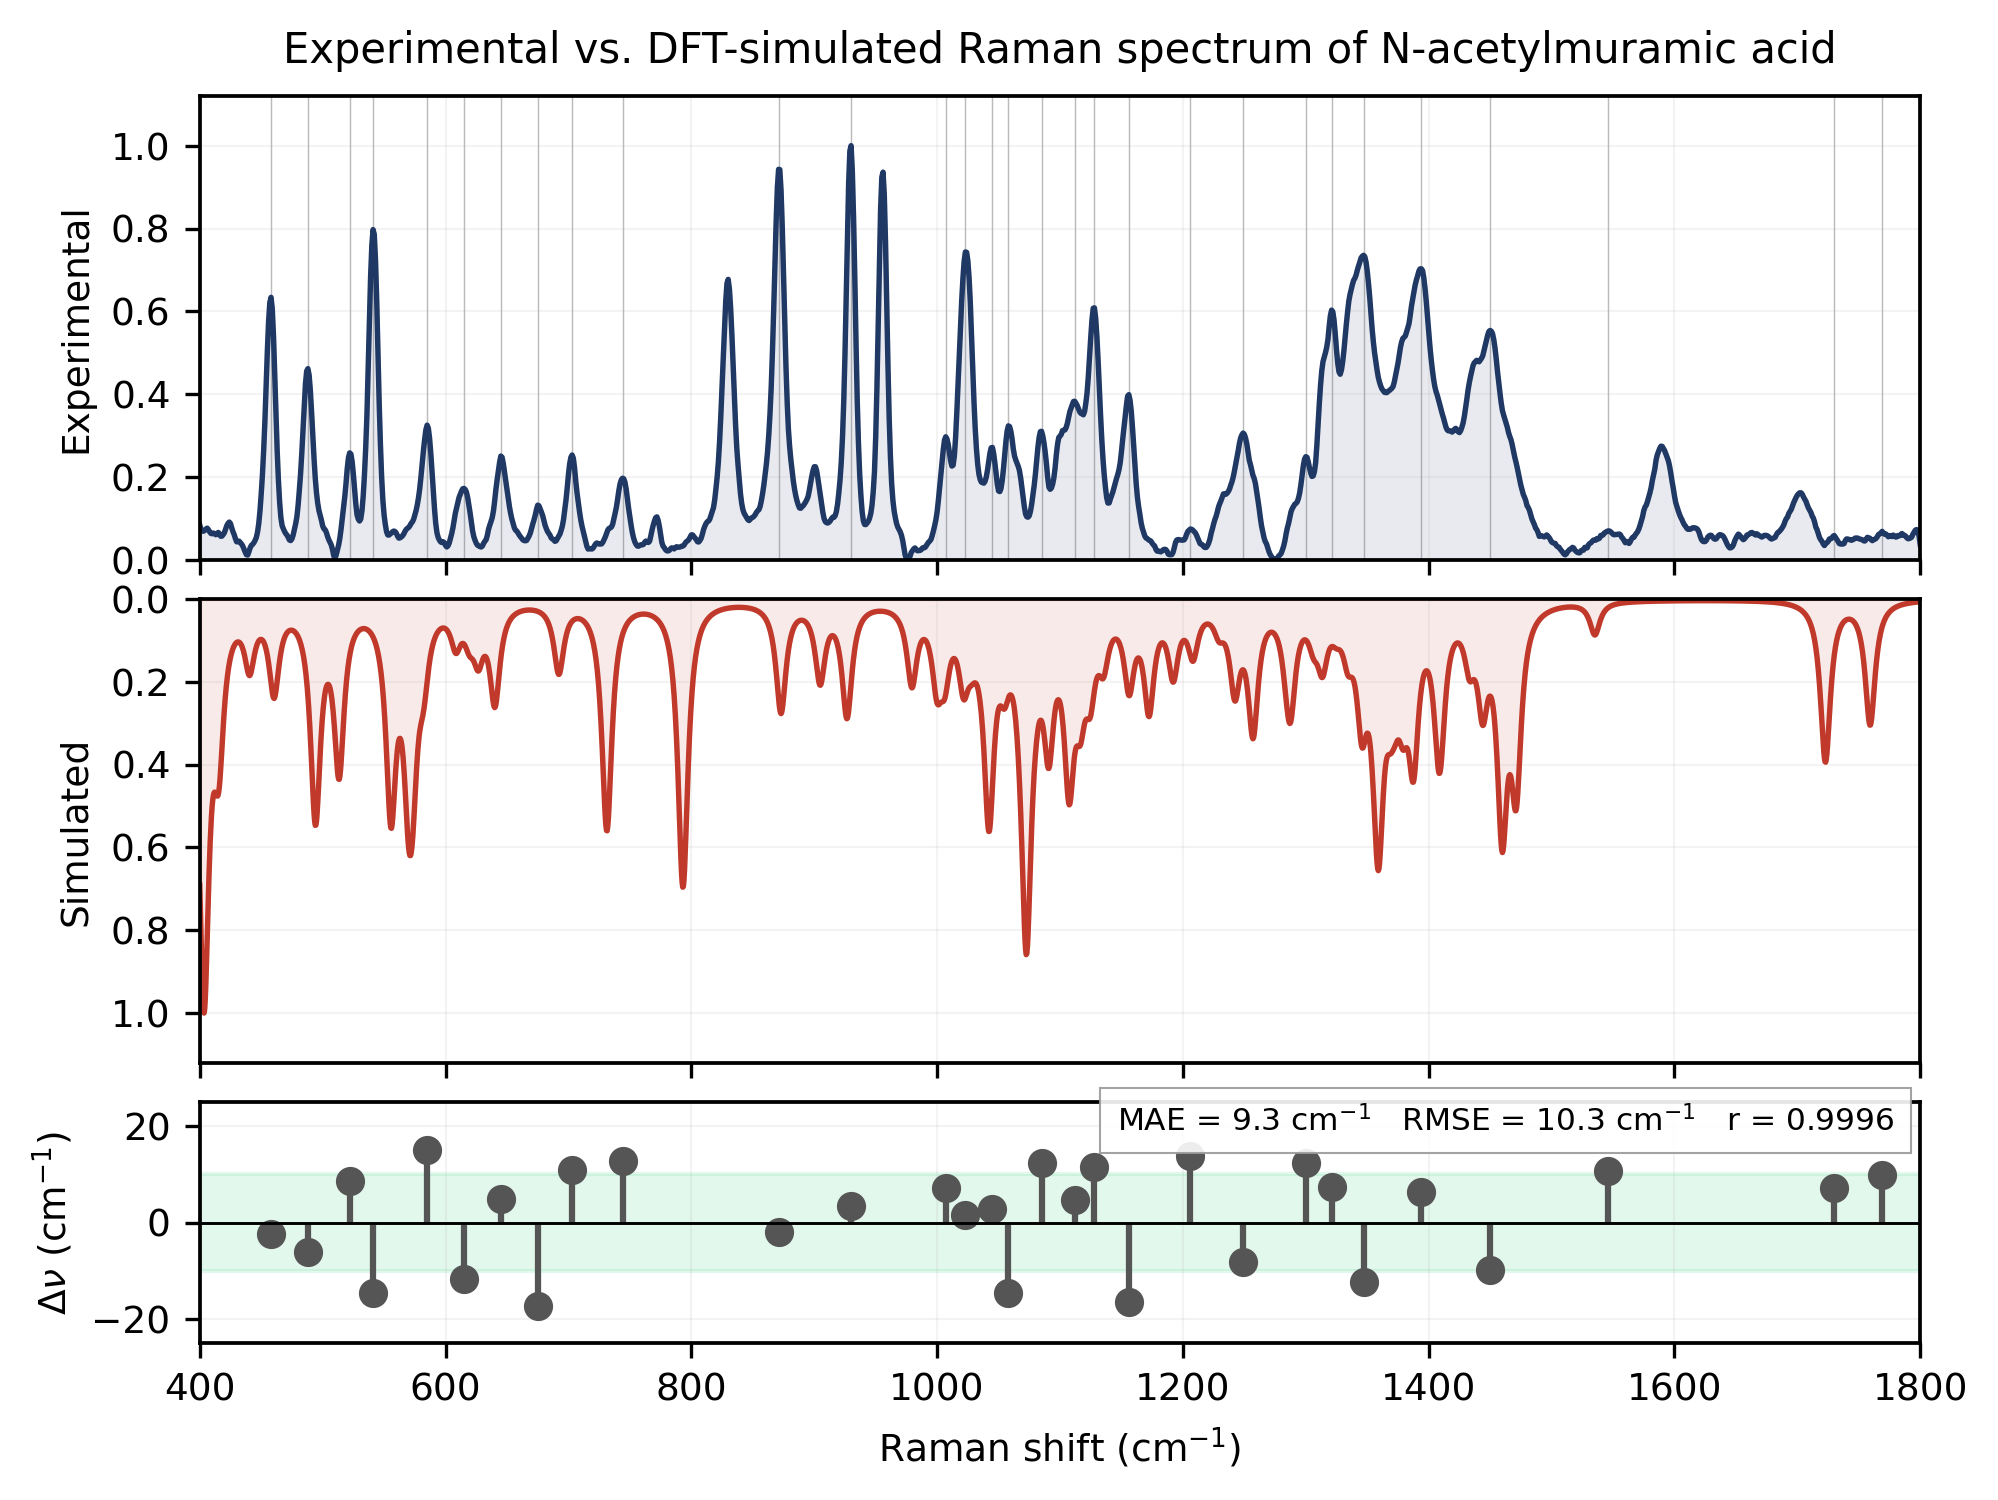
\includegraphics[width=\linewidth]{figures/fig6_overlay.png}
\caption{Comparison of experimental and simulated Raman spectra. Upper panel:
experimental reference spectrum. Middle panel: DFT-simulated spectrum
(inverted). Lower panel: deviation between observed and calculated wavenumbers
for the 30 matched bands; the shaded region denotes $\pm$10~\wn{}.}
\label{fig:overlay}
\end{figure}

Residual discrepancies have three well-understood sources. The calculation
employs the harmonic approximation, whereas real vibrational potentials are
anharmonic, and scaling corrects this only on average. More importantly, the
calculation treats a single isolated molecule in vacuum while the measurement is
of crystalline powder in which extensive intermolecular hydrogen bonding is
present; modes involving hydroxyl, carbonyl and amide groups are most sensitive
to this. Finally, the calculation models the $\beta$ anomer alone whereas the
sample is an anomeric mixture.

\subsection{Vibrational assignments}

The assignments in Table~\ref{tab:comparison} follow the conventional pattern
for pyranose sugars, with two cases where normal-mode decomposition gives a
result that could not be reached from the experimental spectrum alone.

The intense band at 872~\wn{} is reproduced by the calculated mode at
873~\wn{}. Decomposition shows this mode to be dominated by motion of the
hydroxymethyl hydrogens: a single hydrogen bonded to C-6 accounts for 45.9\% of
the mass-weighted displacement and a second for 17.4\%, with the pyranose ring
contributing only 5.0\% and heavy atoms 8.9\% in total. The band is therefore
assigned to out-of-plane wagging of the hydroxymethyl group rather than to ring
breathing, with which it would ordinarily be grouped on frequency alone. The
neighbouring 930~\wn{} band does correspond to a genuine ring-breathing mode
(calculated 927~\wn{}).

The D-lactyl ether at C-3 distinguishes muramic acid from N-acetylglucosamine
and is the structural basis for its bacterial specificity. Its methyl group
contributes to the deformation modes near 1337--1385~\wn{} and to the scissoring
region near 1451--1470~\wn{}, while the associated carboxylic acid gives rise to
the carbonyl stretching feature above 1750~\wn{}. Bands carrying lactyl
character are therefore, in principle, the most promising candidates for
distinguishing muramic acid from other amino sugars in complex spectra, although
in intact peptidoglycan the carboxyl is amide-linked and its spectroscopic
signature correspondingly altered.

The acetamido group produces amide~II near 1544~\wn{}. This grouping is shared
with GlcNAc and is not by itself diagnostic of muramic acid.

\subsection{Unmatched bands}
\label{sec:unmatched}

Eleven observed bands have no calculated counterpart within the matching
tolerance: 772, 830, 956, 1517, 1589, 1637, 1652, 1663, 1702, 1785 and
1797~\wn{}. Nine of these lie above 1500~\wn{}, where the isolated-molecule
model is least applicable.

Two limitations were considered. The first is the anomeric composition of the
sample: the supplier specification leaves the anomeric configuration undefined,
so the measured material is a mixture, whereas the calculation treats the
$\beta$ anomer alone. The 820--980~\wn{} window, which contains the unmatched
830 and 956~\wn{} bands, is where $\alpha$ and $\beta$ pyranoses differ most,
through the anomeric C--H bending and coupled ring deformations.

We tested this explanation directly. The $\alpha$ anomer was optimised and its
Raman spectrum computed at the identical level of theory, from a starting
geometry verified to differ from the $\beta$ structure at the anomeric centre
alone (all five remaining stereocentres identical). The calculation converged
normally with no imaginary frequencies. Considered in isolation the result
appeared to support the hypothesis, five of the eleven unmatched bands falling
within tolerance of an $\alpha$ mode. Two controls show that this apparent
agreement is not meaningful.

First, the unmatched bands are by definition those the $\beta$ calculation
failed to reproduce, so any second set of modes must improve on a baseline of
zero; the comparison is uninformative. Assessed instead across all 41 observed
bands, adding the $\alpha$ modes raises the number matched from 30 to 35. A
control in which the $\beta$ modes were rigidly displaced by a random offset,
preserving their number and spacing but destroying their chemical meaning,
raised the count by $4.3 \pm 2.0$ ($p = 0.46$). The improvement is
indistinguishable from that obtained by doubling the number of available modes
at random, and remains so at every tolerance from $\pm$5 to $\pm$18~\wn{}.
Second, the candidate $\alpha$ modes nearest the 830 and 1517~\wn{} bands carry
0.4\% of the maximum calculated Raman intensity and could not give rise to
observable features, although 830~\wn{} is among the stronger bands measured.

We therefore find no evidence that the anomeric composition of the sample
accounts for the unmatched bands. The $\beta$ anomer is retained as the
reference calculation: it lies 3.1~kcal\,mol$^{-1}$ lower in Gibbs free energy
than the $\alpha$ form at this level of theory, and reproduces the observed
frequencies with a slightly smaller mean absolute deviation (5.7 against
6.4~\wn{}). Both figures refer to single conformers rather than
conformationally averaged ensembles and are indicative only.

The second is the treatment of the solid state. The calculation places the amide
carbonyl stretch at 1723~\wn{}, some 21~\wn{} above the observed 1702~\wn{}
band and outside the matching tolerance. This is the expected direction and
magnitude of error for a gas-phase model: intermolecular hydrogen bonding to the
amide carbonyl in the crystal lowers the stretching frequency substantially, and
no isolated-molecule calculation reproduces that shift. The cluster of features
between 1589 and 1663~\wn{} falls in the same region.

This second explanation is the stronger one, and the $\alpha$ calculation
reinforces it. Neither anomer has any calculated mode between 1535 and
1720~\wn{}, a gap of some 190~\wn{}, yet four reproducible bands are observed
within it at 1589, 1637, 1652 and 1702~\wn{}. Intermolecular hydrogen bonding to
the amide and carboxyl carbonyls in the solid lowers those stretching
frequencies by tens of \wn{}, displacing them into precisely this interval. The
discrepancy is therefore attributable to the isolated-molecule approximation
rather than to the anomeric composition of the sample, and it accounts for the
majority of the unmatched bands.

A further consequence of the sample specification is that the material studied
here differs in solid form from that of the earlier vibrational study, which
examined the crystalline monohydrate \cite{kouach1994}. Band-by-band comparison
with that work should be made with care. Finally, the supplier permits up to one
mole of residual methanol per mole of product. Methanol has a strong Raman band
near 1035~\wn{} together with C--H stretching features at 2835 and 2945~\wn{}.
The spectrometer used here is specified to 2800~\wn{}, so the diagnostic C--H
stretching region is not accessible with this configuration and a contribution
of residual methanol to the 1020--1050~\wn{} region cannot be excluded. Testing
this would require an instrument with extended spectral coverage.

\subsection{The 730~\wn{} region}

The band near 730~\wn{} is among the most prominent features of bacterial SERS
spectra and is widely used in bacterial discrimination, yet its molecular origin
remains contested \cite{premasiri2016origins, kubryk2016origin}. Because
peptidoglycan is a major and bacterium-specific cell-wall constituent, a muramic
acid origin has been considered plausible but could not previously be tested
against a measured isolated-molecule spectrum.

Our calculations place a mode of appreciable Raman activity (5.29~\AA$^4$/amu)
at 731~\wn{} after scaling, apparently consistent with such an assignment.
Decomposition of the calculated displacement vector, however, shows this
interpretation to be incorrect. The mode is dominated by motion of a single
hydrogen atom, contributing 47.9\% of the total mass-weighted displacement,
which the computed connectivity identifies as the hydroxyl proton of the
carboxylic acid group (O--H bond length 0.97~\AA; the parent oxygen is bonded to
the carboxyl carbon at 1.35~\AA, which in turn carries the carbonyl oxygen at
1.21~\AA). The pyranose ring contributes only 0.5\% of the displacement, and
heavy atoms in total 24.0\%. The mode is therefore an out-of-plane deformation
of the carboxylic acid hydroxyl group, $\gamma$(O--H), coupled weakly to lactyl
methyl motion, and not a ring or glycan-backbone vibration.

This distinction has a direct structural consequence. In intact peptidoglycan
the carboxyl group of muramic acid is not free: it is amide-linked to the
L-alanine residue that initiates the peptide stem. The hydroxyl proton
responsible for the calculated 731~\wn{} mode is therefore absent in the
polymer, and the mode cannot contribute to the Raman or SERS spectrum of intact
bacterial cell walls.

Experimentally, the corresponding region of the measured spectrum
(Figure~\ref{fig:region730}) shows only weak features, at 704 and 745~\wn{},
both substantially weaker than the principal ring bands, and neither coincident
with 730~\wn{}.

\begin{figure}[htbp]
\centering
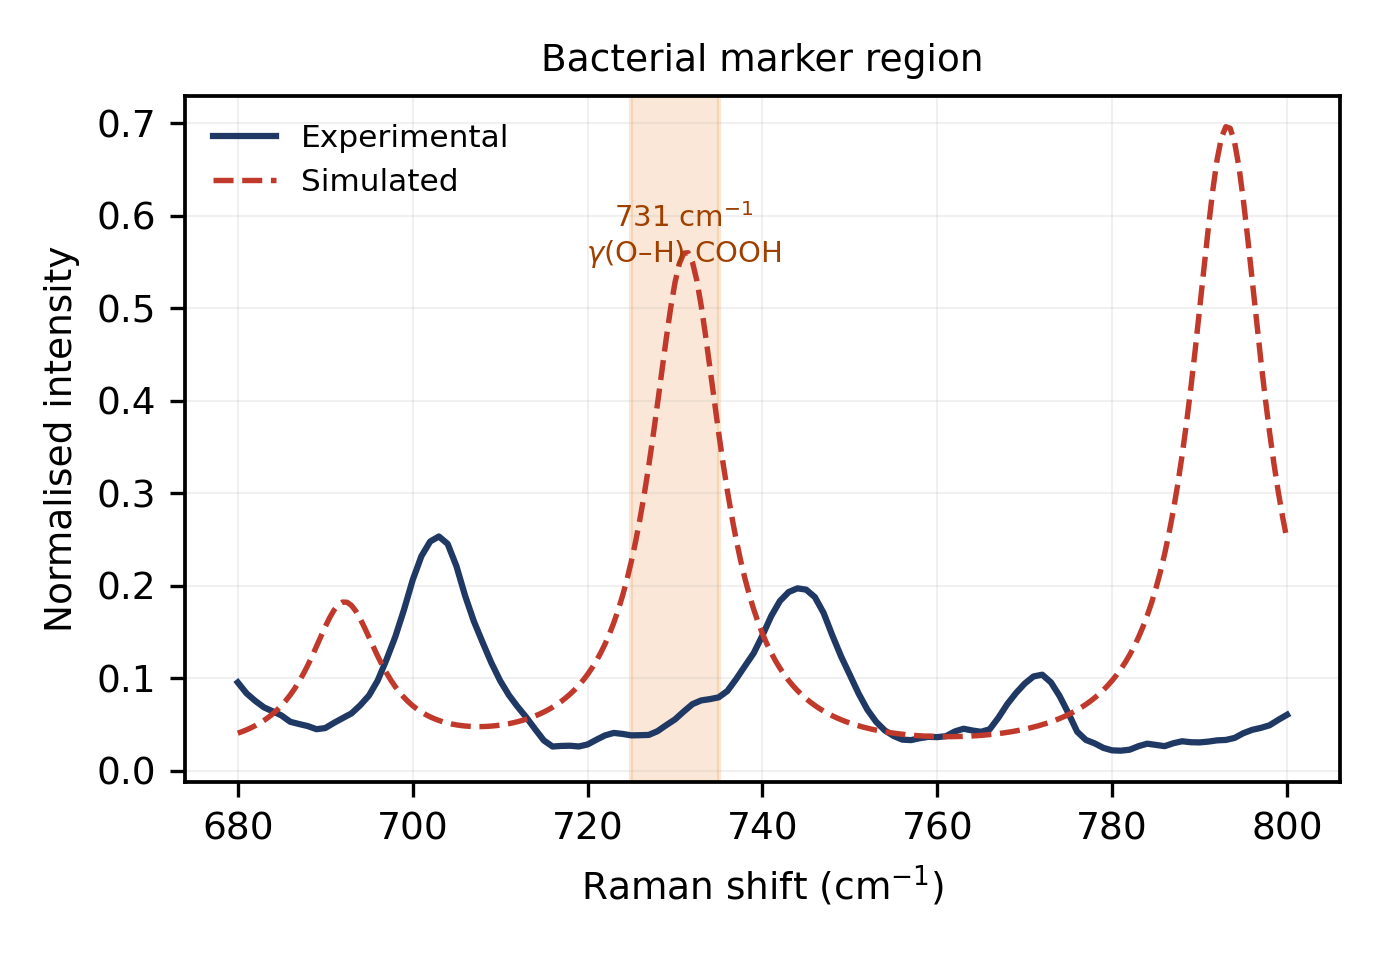
\includegraphics[width=0.62\linewidth]{figures/fig7_region730.png}
\caption{Experimental and simulated spectra in the 680--800~\wn{} region. The
shaded band indicates the disputed 730~\wn{} bacterial marker position. The
calculated mode at 731~\wn{} is shown by normal-mode decomposition to be an
out-of-plane carboxylic acid hydroxyl deformation.}
\label{fig:region730}
\end{figure}

Taken together, these observations provide direct evidence against attributing
the bacterial 730~\wn{} band to muramic acid, and by extension weaken the case
for a peptidoglycan origin. The result is consistent with assignments favouring
adenine-containing species \cite{premasiri2016origins, kubryk2016origin}. We
note the limitations of the argument: the calculation describes the free acid as
an isolated molecule, and a definitive test would require measurements on
muramyl peptides or purified peptidoglycan.

\subsection{Relevance to bacterial Raman and SERS analysis}

The reference spectrum reported here supports the interpretation of bacterial
measurements in three ways. It provides validated band positions against which
candidate peptidoglycan features in whole-cell spectra can be checked. The
assignments identify which bands carry lactyl character and are therefore
capable in principle of distinguishing muramic acid from N-acetylglucosamine.
And the 730~\wn{} analysis removes one candidate explanation for a widely used
bacterial marker band, narrowing the interpretive space.

For SERS applications these data provide the necessary non-enhanced baseline.
Comparison of enhanced with non-enhanced spectra is what permits adsorption
geometry to be inferred from surface selection rules, and such comparison
requires a reliable reference of this kind. The photostability limits reported
in Section~\ref{sec:photostab} are also directly relevant, since plasmonic
substrates concentrate the incident field and can lower the damage threshold
considerably.

We emphasise that these measurements are of dry powder, and that extrapolation
to bacterial suspensions, and still more to clinical matrices, requires separate
validation.

%======================================================================
\section{Conclusions}
%======================================================================

A reference Raman spectrum of isolated N-acetylmuramic acid has been established
from 22 independent measurements on fresh sample and compared with harmonic
frequencies computed at the B3LYP-D3BJ/6-311++G(d,p) level. Forty-one
reproducible bands were identified in the 400--1800~\wn{} fingerprint region, of
which thirty were assigned to calculated normal modes with a mean absolute
deviation of 9.3~\wn{} and a correlation coefficient of 0.9996.

Photostability measurements across 227 spectra define a working envelope for
this material at 785~nm: the spectrum is unchanged over ten consecutive scans at
90\% laser power with 30~s integration, but the sample is destroyed at the same
power with 60~s integration.

Normal-mode decomposition resolved two assignments not accessible from the
experimental spectrum alone. The intense 872~\wn{} band arises from
hydroxymethyl wagging rather than ring breathing. The calculated mode in the
disputed 730~\wn{} bacterial marker region arises from out-of-plane deformation
of the carboxylic acid hydroxyl group, with negligible ring character; since
this proton is absent in intact peptidoglycan, the result argues against a
muramic acid origin for the bacterial 730~\wn{} band.

Extension of this work to N-acetylglucosamine, to the $\alpha$ anomer, to
muramyl peptides and to surface-enhanced measurements would allow the
peptidoglycan contribution to bacterial Raman spectra to be characterised more
completely.

%======================================================================
\begin{table}[htbp]
\centering
\caption{Observed and calculated Raman wavenumbers of isolated N-acetylmuramic
acid with proposed vibrational assignments. Calculated values are scaled (0.980
below 1800~\wn{}). $\Delta = \nu_{\mathrm{exp}} - \nu_{\mathrm{calc}}$.
Reproducibility is the percentage of the 22 independent spectra in which the
band was detected. $\nu$: stretching; $\delta$: in-plane bending; $\gamma$:
out-of-plane bending. $^{\dagger}$Tentative: satisfies only one of the two
signal-to-noise criteria of Section~2.6.}
\label{tab:comparison}
\small
\begin{tabular}{rrrrrrp{4.4cm}}
\toprule
Exp. & Calc. & $\Delta$ & Raman act. & Rel. & Repro. & Proposed assignment \\
(\wn{}) & (\wn{}) & (\wn{}) & (\AA$^4$/amu) & int. & (\%) & \\
\midrule
458 & 460.5 & -2.5 & 1.0 & 0.63 & 100 & Skeletal bending / ring torsion \\
488 & 494.2 & -6.2 & 2.8 & 0.46 & 100 & Skeletal bending / ring torsion \\
522 & 513.4 & +8.6 & 2.3 & 0.26 & 100 & Skeletal bending / ring torsion \\
541 & 555.6 & -14.6 & 3.2 & 0.80 & 100 & Skeletal bending / ring torsion \\
585 & 570.0 & +15.0 & 2.3 & 0.33 & 100 & Skeletal bending / ring torsion \\
615 & 626.7 & -11.7 & 0.8 & 0.17 & 100 & Skeletal deformation + $\delta$(C--C--O) \\
645 & 640.1 & +4.9 & 1.9 & 0.25 & 100 & Skeletal deformation + $\delta$(C--C--O) \\
675 & 692.2 & -17.2 & 1.5 & 0.13 & 95 & Skeletal deformation + $\delta$(C--C--O) \\
703 & 692.2 & +10.8 & 1.5 & 0.25 & 100 & Skeletal deformation + $\delta$(C--C--O) \\
744 & 731.3 & +12.7 & 5.3 & 0.20 & 100 & $\gamma$(O--H) carboxylic acid out-of-plane \\
772 & -- & -- & -- & 0.10 & 100 & unmatched \\
830 & -- & -- & -- & 0.68 & 100 & unmatched \\
871 & 873.0 & -2.0 & 3.2 & 0.94 & 100 & $\gamma$(CH$_2$) hydroxymethyl wagging \\
930 & 926.7 & +3.3 & 3.6 & 1.00 & 100 & Ring breathing / $\nu$(C--C--O) \\
956 & -- & -- & -- & 0.94 & 100 & unmatched \\
1007 & 999.9 & +7.1 & 2.4 & 0.30 & 100 & Ring breathing / $\nu$(C--C--O) \\
1023 & 1021.5 & +1.5 & 2.3 & 0.74 & 100 & $\nu$(C--O) + $\delta$(C--O--H) \\
1045$^{\dagger}$ & 1042.2 & +2.8 & 7.7 & 0.27 & 100 & $\nu$(C--O) + $\delta$(C--O--H) \\
1058 & 1072.7 & -14.7 & 12.4 & 0.32 & 100 & $\nu$(C--O) + $\delta$(C--O--H) \\
1085$^{\dagger}$ & 1072.7 & +12.3 & 12.4 & 0.31 & 100 & $\nu$(C--O) + $\delta$(C--O--H) \\
1112 & 1107.4 & +4.6 & 6.6 & 0.38 & 100 & $\nu$(C--O) + $\delta$(C--O--H) \\
1128 & 1116.6 & +11.4 & 3.1 & 0.61 & 100 & $\nu$(C--O) + $\delta$(C--O--H) \\
1156 & 1172.4 & -16.4 & 4.4 & 0.40 & 100 & $\nu$(C--O) + $\delta$(C--O--H) \\
1206$^{\dagger}$ & 1192.1 & +13.9 & 3.0 & 0.07 & 95 & $\nu$(C--O) + $\delta$(C--O--H) \\
1249 & 1257.1 & -8.1 & 6.0 & 0.31 & 100 & $\delta$(C--H) + $\nu$(C--O) coupled \\
1300$^{\dagger}$ & 1287.6 & +12.4 & 4.5 & 0.25 & 95 & $\delta$(C--H) + $\nu$(C--O) coupled \\
1321 & 1313.6 & +7.4 & 2.7 & 0.60 & 100 & $\delta$(C--H) + $\nu$(C--O) coupled \\
1347 & 1359.3 & -12.3 & 11.0 & 0.73 & 100 & $\delta$(C--H) / $\delta$s(CH$_3$) umbrella \\
1394 & 1387.6 & +6.4 & 7.8 & 0.70 & 100 & $\delta$(C--H) / $\delta$s(CH$_3$) umbrella \\
1450 & 1459.7 & -9.7 & 7.6 & 0.55 & 95 & $\delta$(CH$_2$) scissoring / $\delta$as(CH$_3$) \\
1517$^{\dagger}$ & -- & -- & -- & 0.03 & 100 & unmatched \\
1546 & 1535.2 & +10.8 & 2.2 & 0.07 & 77 & Amide II: $\delta$(N--H) + $\nu$(C--N) \\
1589 & -- & -- & -- & 0.27 & 91 & unmatched \\
1637$^{\dagger}$ & -- & -- & -- & 0.06 & 91 & unmatched \\
1652$^{\dagger}$ & -- & -- & -- & 0.06 & 91 & unmatched \\
1663$^{\dagger}$ & -- & -- & -- & 0.07 & 77 & unmatched \\
1702 & -- & -- & -- & 0.16 & 100 & unmatched \\
1730$^{\dagger}$ & 1722.8 & +7.2 & 12.8 & 0.06 & 100 & Amide I: $\nu$(C=O) \\
1769 & 1759.2 & +9.8 & 10.2 & 0.07 & 82 & $\nu$(C=O) carboxylic acid \\
1785 & -- & -- & -- & 0.06 & 68 & unmatched \\
1797 & -- & -- & -- & 0.07 & 82 & unmatched \\
\bottomrule
\end{tabular}
\end{table}

%======================================================================
\section*{CRediT authorship contribution statement}
\textbf{Sukesh P:} Conceptualisation, Methodology, Investigation, Formal
analysis, Software, Visualisation, Writing --- original draft.
\authorcheck{Add co-authors and their contributions.}

\section*{Declaration of competing interest}
The authors declare no competing financial interests or personal relationships
that could have influenced the work reported in this paper.

\section*{Data availability}
Processed Raman spectra, the complete list of calculated frequencies and Raman
activities, and the optimised molecular geometry are provided as Supplementary
Material. Raw spectra and Gaussian output files are available from the
corresponding author on request.
\authorcheck{Consider depositing the full archive in Zenodo and citing the DOI.}

\section*{Acknowledgements}
The author thanks the Indian Institute of Technology Jodhpur for access to Raman
spectroscopy and computational facilities.
\authorcheck{Add supervisor, colleagues, funding sources and grant numbers.}

%======================================================================
\begin{thebibliography}{99}

\bibitem{wang2022bacteria}
Y.~Wang, et~al., Bacteria detection: from powerful SERS to advanced
spectroscopic techniques, Biosensors 12 (2022) 210.

\bibitem{ma2024ecoli}
D.~Ma, et~al., \emph{Escherichia coli} research on Raman measurement mechanism
and diagnostic model, Vibrational Spectroscopy 132 (2024) 103670.

\bibitem{vollmer2008}
W.~Vollmer, D.~Blanot, M.~A.~de~Pedro, Peptidoglycan structure and architecture,
FEMS Microbiology Reviews 32 (2008) 149--167.

\bibitem{she1974raman}
C.~Y.~She, et~al., Laser Raman spectra of glucosamine and related amino sugars,
Spectrochimica Acta Part A 30 (1974) 1387--1395.

\bibitem{kaminsky2020saccharides}
J.~Kaminsk\'y, et~al., Simulation of Raman and Raman optical activity spectra of
saccharides in water, Physical Chemistry Chemical Physics 22 (2020) 12345--12356.

\bibitem{kouach1994}
M.~Kouach, et~al., Vibrational spectra and harmonic dynamics of
N-acetyl-muramic acid monohydrate, Journal of Molecular Structure 317 (1994)
153--166.
\authorcheck{VERIFY authors, volume and pages against the actual paper}

\bibitem{premasiri2016origins}
W.~R.~Premasiri, et~al., The biochemical origins of the surface-enhanced Raman
spectra of bacteria, Applied Spectroscopy 70 (2016) 1136--1149.

\bibitem{kubryk2016origin}
P.~Kubryk, et~al., The origin of the band at around 730~cm$^{-1}$ in the SERS
spectra of bacteria, Analyst 141 (2016) 3986--3994.

\bibitem{gaussian16}
M.~J.~Frisch, et~al., Gaussian~16, Revision C.01, Gaussian, Inc.,
Wallingford CT, 2019.

\bibitem{becke1993}
A.~D.~Becke, Density-functional thermochemistry. III. The role of exact
exchange, Journal of Chemical Physics 98 (1993) 5648--5652.

\bibitem{lee1988}
C.~Lee, W.~Yang, R.~G.~Parr, Development of the Colle--Salvetti
correlation-energy formula into a functional of the electron density, Physical
Review B 37 (1988) 785--789.

\bibitem{grimme2011}
S.~Grimme, S.~Ehrlich, L.~Goerigk, Effect of the damping function in dispersion
corrected density functional theory, Journal of Computational Chemistry 32
(2011) 1456--1465.

\bibitem{eilers2005}
P.~H.~C.~Eilers, H.~F.~M.~Boelens, Baseline correction with asymmetric least
squares smoothing, Leiden University Medical Centre Report, 2005.

\bibitem{savitzky1964}
A.~Savitzky, M.~J.~E.~Golay, Smoothing and differentiation of data by simplified
least squares procedures, Analytical Chemistry 36 (1964) 1627--1639.

% <<EXPAND to 30-45 references before submission.>>
% Priority: Frosch et al. (scaling factors); 4-6 recent bacterial SERS papers;
% 3-4 combined experimental+DFT vibrational studies; further amino-sugar Raman
% literature; laser-damage / photodegradation studies of carbohydrates.

\end{thebibliography}
\end{document}
